%---------------------------------------------------------------%
\documentclass[a4paper]{jarticle}
%---------------------------------------------------------------%
% プリアンブル
%---------------------------------------------------------------%
\usepackage{rpstyle}
\usepackage{amsmath,amsthm,amssymb}
\usepackage{wrapfig}
\usepackage{epic, eepic}
\usepackage{ascmac}
\usepackage{verbatim}
\usepackage{multicol}
\usepackage{subfigure}
\usepackage{url}
\usepackage{here}
%\usepackage{arydshln}
% dvioutで確認する場合は以下を有効にする
%\usepackage[dvips]{graphicx,color}
% pdf化する場合は以下を有効にする
\usepackage[dvipdfmx]{graphicx,color}

\def\degC{\kern-.2em\r{}\kern-.3em C}
\def\degree{\kern-.2em\r{}\kern-.3em}
%---------------------------------------------------------------%%
% タイトル&著者
\title{(イ)卒業研究に向けた先行研究の調査結果}
\author{鷲尾 優作}
%
% 報告日
\date{Feb 21, 2023}
%
% 概要
\abstract{
本稿では,卒業研究に向けた先行研究の調査結果をまとめる.ここでは,卒業研究として積雪寒冷地域における自動運転の実現に向けた
研究を想定し,先行して実施されている研究を調査した.国内外ともに積雪寒冷地域にフォーカスした研究は少なかったが,
戦略的基盤技術高度化支援事業「積雪寒冷地域の交通弱者移動支援のための雪道走行を可能とする自動運転技術の開発」が非常に有用な情報であることがわかった.
}
%
% キーワード
\keyword{自動運転, 積雪寒冷地未対応課題, 冬型事故, わだち事故, LiDAR}
%
% 書式の再設定
\newcommand{\sline}{\rule{17.5cm}{0.5mm}}
%
\begin{document}
\maketitle
%
%---------------------------------------------------------------%
\section{はじめに}
%
現在、各国で自動運転の実用化に向けた開発競争が激化している.
しかしながら、現行のシステムは利用者の多い都市部を中心に実験・データ収集を実施している為、
積雪寒冷地域において自動走行の精度が低下する問題が指摘されている(積雪寒冷地未対応課題)

積雪寒冷地域における自動運転の実現に向けた技術開発を行うことを想定し,先行して実施されている研究を調査した.
%
%---------------------------------------------------------------%
\section{報告内容}
%
\subsection{調査背景}
文献\cite{yahoo-sonnahashiri:online},「そんな走りで大丈夫か 自動運転で雪道を走るテスラが不安定すぎる ふらふらとまっすぐ走れない様子が恐ろしい」では,
テスラの自動運転車「モデル3」が雪道を走る様子が不安定であると指摘されている.、テスラが2022年11月から試験的に配布している自動運転機能「FSD」を用いた実験であり,
正式リリースされているシステムではないものの,積雪寒冷地域においては自動運転の精度が低下ことがわかった.

この課題に興味を持ったため,卒業研究のテーマとして積雪寒冷地域における自動運転の実現に向けた技術開発について調査する.

\subsection{国内における積雪寒冷を原因とする事故について}
文献\cite{blizzard52:online}より,Fig.\ref{21}を示す.

\begin{figure}[H]
  \centering
  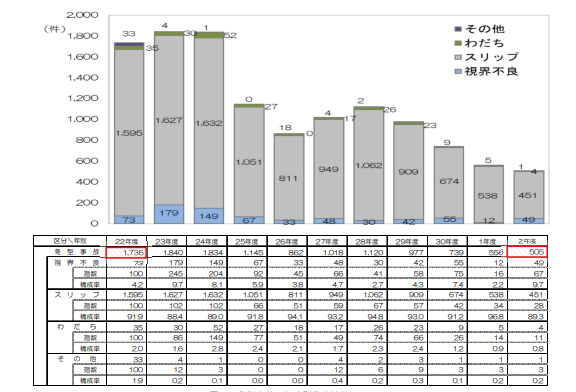
\includegraphics[width=0.4\linewidth]{picture/21.png}
  \caption{冬型事故の年度別発生件数}
  \label{21}
\end{figure}

資料から,北海道内では平均して年間約1,000件の冬型事故が発生していることがわかる.
また,冬型事故のほとんどはスリップによるものであり,凍結の危険性がわかる.

\subsection{積雪寒冷地域における自動運転の実現に向けた研究}
積雪寒冷地域における自動運転の実現に向けた研究は国内外ともに少ない.
積極的に研究を進めているのは,米フォード,VTTフィンランド技術研究センター,北海道大学といった寒冷地に拠点を持つ
限られたチームのみである.文献\cite{cobby:online}は,これら研究機関の研究動機や積雪寒冷地域での
自動運転が難しくなる理由をわかりやすくまとめており,参考になる.

\subsection{自動運転のための道路の積雪の認識に関する研究}
積雪寒冷地域において自動運転を行うためには,そもそも雪を認識する必要がある.
しかしながら,降雪中はセンサが大気中の雪も認識してしまうことや自己位置推定に必要なランドマークが認識できなくなるといった問題が生じる.
文献\cite{ja83:online}では,測量用の3Dレーザスキャナを用いて認識を行う研究を行っている.
基本的に認識は可能であるが,鉛直方向の位置合わせに大きな課題があることが示されている.

\subsection{自動運転バスは雪道を走れるのか 実験}
文献\cite{bass:online}は,ソフトバンク子会社のBOLDLYが本来雪道を想定していないフランス製自動運転バスを
積雪寒冷地域で走らせる実験を行った記事である.

積雪時には問題なく走行できるが,降雪中には雪に反応し走行が不安定になる結果となっている.

\begin{figure}[H]
  \centering
  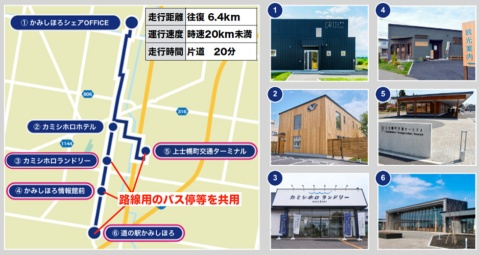
\includegraphics[width=0.4\linewidth]{picture/02.jpg}
  \caption{冬型事故の年度別発生件数} 
  \label{02}
\end{figure}

\section{積雪寒冷地域の交通弱者移動支援のための雪道走行を可能とする自動運転技術の開発}
文献\cite{2910102026:online}は,北海道の研究チームが積雪寒冷地域での自動運転における技術開発を補助金を使って実施した報告書である.
この研究では,「雪道対応SLAM」,「雪道対応セマンティックセグメンテ=ション」,「雪道対応センサフュージョン」
の3つを柱に自己位置推定技術を開発しており,技術的な面では現在把握できている資料の中で最も参考になるものである.

先述した鉛直方向での自己位置推定について問題については,Voxelを用いる障害物検知を組み合わせる手法が提案されていた.

\begin{figure}[H]
  \centering
  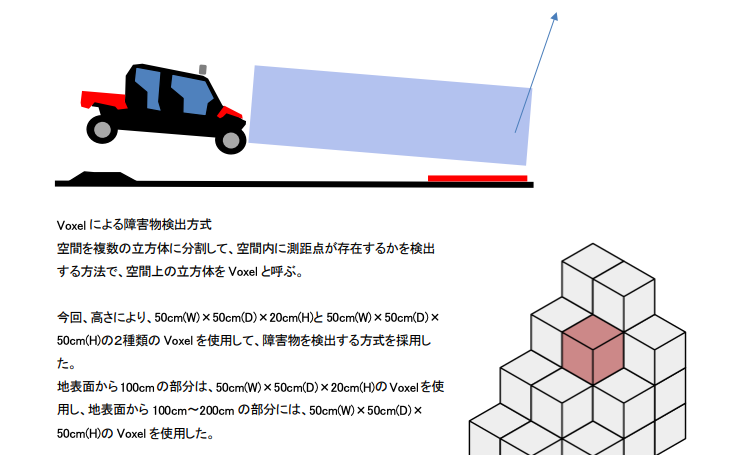
\includegraphics[width=0.5\linewidth]{picture/voxel.png}
  \caption{Voxel投票による障害物検知} 
  \label{voxel}
\end{figure}

また,Kerasを用いたセグメンテーションとハフ変換を組み合わせ,走行可能な場所を判定する手法も提案されている.
この応用で他の方法を組み合わせることで,走行可能領域中の轍や障害物の分布を詳しく調べることができるかもしれないと考えられる.

\begin{figure}[H]
  \centering
  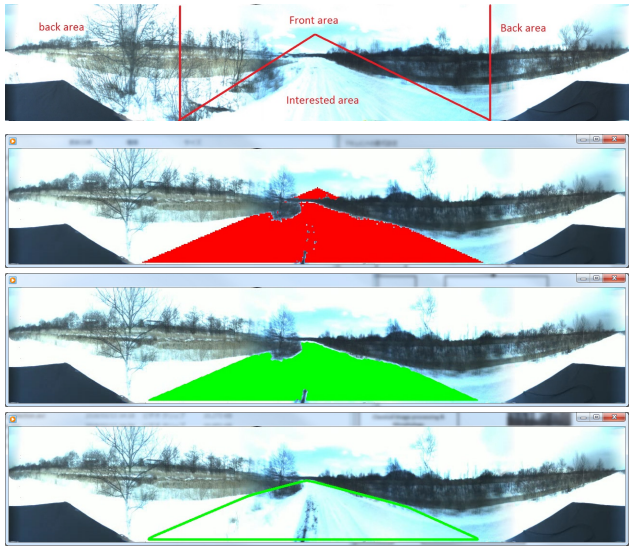
\includegraphics[width=0.5\linewidth]{picture/soukou.png}
  \caption{走行可能領域の判定} 
  \label{voxel}
\end{figure}

%
%---------------------------------------------------------------%
\section{おわりに}
%
以上の調査結果をもとに,今後は具体的な研究計画を作成する.
「積雪寒冷地域の交通弱者移動支援のための雪道走行を可能とする自動運転技術の開発」は他にも赤外センサー,Lidar,SegNetなど
いくつかの手法を試しており,熟読の必要がある.
現時点では,轍や凍結路面等の認識に関心がある.
%
%---------------------------------------------------------------%
%
\bibliographystyle{junsrt}
\bibliography{refs}
%
\end{document}
